\section{Multivariate normal distribution ($N(\mu, \Sigma)$)}

\begin{figure}[H]
    \centering
    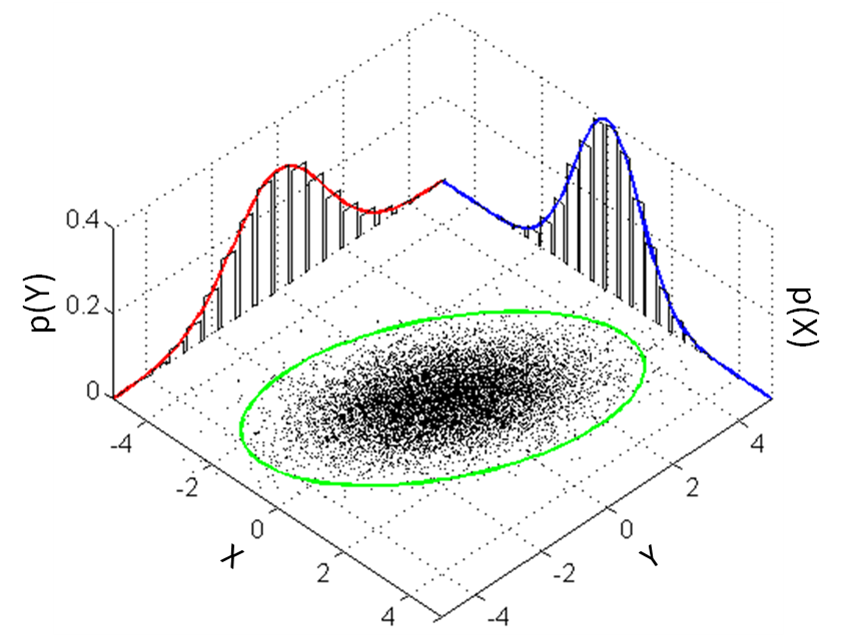
\includegraphics[
        width=\linewidth,
        height=6cm,
        keepaspectratio,
    ]{images/distributions/MultivariateNormal-pdf.png}
    \caption{Multivariate normal distribution: PDF \cite{wiki/Multivariate_normal_distribution}}
\end{figure}


\subsection{PDF}

\begin{enumerate}
    \item
    $
        \mathcal{N}(\bm{x}|\bm{\mu}, \bm{\Sigma})
        = \dfrac{1}{(2\pi)^{D/2} \dabs{\bm{\Sigma}}^{1/2}} \,
        \exp\dParenBrac{
            -\dfrac{1}{2}
            (\bm{x} - \bm{\mu})^\top \bm{\Sigma}^{-1} (\bm{x} - \bm{\mu})
        }
    $
    \hfill \cite{ml/book/Pattern-Recognition-And-Machine-Learning/Christopher-M-Bishop}
    \\[0.2cm]
    .\hfill
    $\bm{x}, \bm{\mu} \in \mbbR^D$
    \hfill
    $\bm{\Sigma} \in \mbbR^{D \times D}$
    \hfill
    $\dabs{\bm{\Sigma}} = \det(\bm{\Sigma}) \in \mbbR$
    \hfill \cite{ml/book/Pattern-Recognition-And-Machine-Learning/Christopher-M-Bishop}

    \item when $X$ and $Y$ are marginally normally distributed, there are different ways of creating dependencies between $X$ and $Y$ that are different from the bivariate PDF
    \hfill \cite{statistics/book/Statistics-for-Data-Scientists/Maurits-Kaptein}
    \\
    Even if two random variables $X$ and $Y$ each individually follow a normal distribution (i.e., their marginals are normal), the way in which they are dependent or correlated can vary.
    That is, their joint distribution doesn't have to be the bivariate normal distribution
    \hfill \cite{common/online/chatgpt}
\end{enumerate}



\subsection{Bivariate Normal Distributions}

\begin{enumerate}[series=binvar-normal]
    \item PDF:
    $
        f (x, y)
        = \dfrac{1}{ 2\pi\sigma_X \sigma_Y \sqrt{1 - \rho^2} }
        \exp \dParenBrac{
            - \dfrac{z^2_1 - 2\rho z_1z_2 + z^2_2 }{2(1 - \rho^2)}
        }
    $
    \hfill \cite{statistics/book/Statistics-for-Data-Scientists/Maurits-Kaptein}
    \begin{enumerate}
        \item $z_1 = \dfrac{x - \mu_X}{\sigma_X}$: standardized normal variable for $X$
        \hfill \cite{statistics/book/Statistics-for-Data-Scientists/Maurits-Kaptein}

        \item $z_2 = \dfrac{y - \mu_Y}{\sigma_Y}$: standardized normal variable for $Y$
        \hfill \cite{statistics/book/Statistics-for-Data-Scientists/Maurits-Kaptein}

        \item $\rho$: \textbf{correlation coefficient} and is contained within the interval $[-1, 1]$.
        \hfill \cite{statistics/book/Statistics-for-Data-Scientists/Maurits-Kaptein}

        \item When $\rho = 0$, the normal random variables $X$ and $Y$ are \textbf{independent}
        \hfill \cite{statistics/book/Statistics-for-Data-Scientists/Maurits-Kaptein}

        \item when $\rho \neq 0$, the normal random variables $X$ and $Y$ are \textbf{dependent}
        \hfill \cite{statistics/book/Statistics-for-Data-Scientists/Maurits-Kaptein}
    \end{enumerate}

    \item 
    $
        \begin{aligned}
            \tCov[X, Y] 
            & = \mbbE[(X - \mu _X )(Y - \mu _Y )]
            = \sigma _X \sigma _Y \mbbE[Z_1 Z_2] \\
            &= \sigma _X \sigma _Y \dint^\infty_{-\infty} \dint^\infty_{-\infty} z_1z_2 \dfrac{1}{2\pi (1-\rho^2)} \exp \dParenBrac{ - \dfrac{z^2_1-2\rho z_1 z_2+z^2_2} {2(1-\rho^2)} } dz_1\ dz_2\\
            &= \sigma _X \sigma _Y \dint^\infty_{-\infty} z_2 \dfrac{1}{\sqrt{2\pi}}  \exp \dParenBrac{ - \dfrac{z^2_2} {2} } \dint^\infty_{-\infty} z_1 \dfrac{1}{\sqrt{2\pi (1-\rho^2)}} \exp \dParenBrac{ - \dfrac{(z_1-\rho z_2)^2 }{2(1-\rho^2)} } dz_1\ dz_2 \\
            &= \sigma_X \sigma_Y \dint^\infty_{-\infty} \rho z^2_2 \dfrac{1}{\sqrt{2\pi}}  \exp \dParenBrac{ - \dfrac{z^2_2}{ 2} } dz_2 
            = \rho \sigma_X \sigma_Y
        \end{aligned}
    $
    \hfill \cite{statistics/book/Statistics-for-Data-Scientists/Maurits-Kaptein}

    \item The distribution function of any linear combination of $X$ and $Y$ , say $a X + bY$ , has a normal distribution function with mean $\mu = a\mu_X + b\mu_Y$ and variance $\sigma ^2 = a^2\sigma ^2_X + 2ab\rho \sigma _X \sigma _Y + b^2\sigma ^2_Y$ .
    \hfill \cite{statistics/book/Statistics-for-Data-Scientists/Maurits-Kaptein}

    \item Pearson’s Correlation Coefficient: $\rho_P = CORR(X, Y) = \rho$
    \hfill \cite{statistics/book/Statistics-for-Data-Scientists/Maurits-Kaptein}
\end{enumerate}


\begin{multicols}{2}
\begin{enumerate}[resume*=binvar-normal]
    \item $\mbbE[X] = \mu_X$
    \hfill \cite{statistics/book/Statistics-for-Data-Scientists/Maurits-Kaptein}
    
    \item $\mbbE[Y] = \mu_Y$
    \hfill \cite{statistics/book/Statistics-for-Data-Scientists/Maurits-Kaptein}
    
    \item $\mbbV[X] = \sigma^2_X$
    \hfill \cite{statistics/book/Statistics-for-Data-Scientists/Maurits-Kaptein}
    
    \item $\mbbV[Y] = \sigma^2_Y$
    \hfill \cite{statistics/book/Statistics-for-Data-Scientists/Maurits-Kaptein}
\end{enumerate}
\end{multicols}




\subsection{Farlie-Gumbel-Morgenstern (FGM) Family of Distributions}

\begin{enumerate}
    \item  if we choose $F_X$ and $F_Y$ normal CDFs, we have created a bivariate CDF for $X$ and $Y$ that has marginal normal CDFs, but which is \textbf{not equal} to the bivariate normal PDF given by the bivariate PDF:
    \hfill \cite{statistics/book/Statistics-for-Data-Scientists/Maurits-Kaptein}
    \\[0.3cm]
    .\hfill
    $
        f (x, y)
        = \dfrac{1}{ 2\pi\sigma_X \sigma_Y \sqrt{1 - \rho^2} }
        \exp \dParenBrac{
            - \dfrac{z^2_1 - 2\rho z_1z_2 + z^2_2 }{2(1 - \rho^2)}
        }
    $
    \hfill \cite{statistics/book/Statistics-for-Data-Scientists/Maurits-Kaptein}
\end{enumerate}





\subsection{Mixtures of Probability Distributions}

\subsubsection{Conditionally independent}

\begin{enumerate}
    \item Assume that $Z$ is normally distributed with mean $\mu_Z$ and variance $\sigma^2_Z$ and conditional PDFs $f_{X|Z} (x|z)$ and $f_{X|Z} (x|z)$ are given by $f_{X|Z} (x|z) = \dfrac{1}{\sigma_1} \phi\dParenBrac{\dfrac{x - \mu_1 - z}{\sigma_1}}$ and $f_{Y |Z} (y|z) = \dfrac{1}{\sigma_2} \phi\dParenBrac{\dfrac{y - \mu_2 - z}{\sigma_2}}$ , with $\phi$ the standard normal PDF, then:
    \hfill \cite{statistics/book/Statistics-for-Data-Scientists/Maurits-Kaptein}
    \\
    .\hfill
    $
        f (x, y)
        = \dfrac{1}{ 2\pi\sigma_X \sigma_Y \sqrt{1 - \rho^2} }
        \exp \dParenBrac{
            - \dfrac{z^2_1 - 2\rho z_1z_2 + z^2_2 }{2(1 - \rho^2)}
        }
    $
    \hfill \cite{statistics/book/Statistics-for-Data-Scientists/Maurits-Kaptein}
    \\
    with
    \begin{multicols}{2}
    \begin{enumerate}
        \item $\mu_X = \mu_Z + \mu_1$
        \hfill \cite{statistics/book/Statistics-for-Data-Scientists/Maurits-Kaptein}

        \item $\mu_Y = \mu_Z + \mu_2$
        \hfill \cite{statistics/book/Statistics-for-Data-Scientists/Maurits-Kaptein}

        \item $\sigma^2_X = \sigma^2_Z + \sigma^2_1$
        \hfill \cite{statistics/book/Statistics-for-Data-Scientists/Maurits-Kaptein}

        \item $\sigma^2_Y = \sigma^2_Z + \sigma^2_2$
        \hfill \cite{statistics/book/Statistics-for-Data-Scientists/Maurits-Kaptein}

        \item $\rho = \dfrac{\sigma^2_Z }{\sqrt{(\sigma^2_Z + \sigma^2_1 )(\sigma^2_Z + \sigma^2_2 )}}$
        \hfill \cite{statistics/book/Statistics-for-Data-Scientists/Maurits-Kaptein}
    \end{enumerate}
    \end{multicols}
\end{enumerate}












\subsection{Summary}

\begin{enumerate}

    \item
    \textbf{Notation}:
    $  {\displaystyle {\mathcal {N}}({\boldsymbol {\mu }},\,{\boldsymbol {\Sigma }})} $
    \hfill \cite{wiki/Multivariate_normal_distribution}

    \item
    \textbf{Parameters}:
    \begin{enumerate}
        \item $\bm{\mu} \in \mbbR^k$ — location
        \hfill \cite{wiki/Multivariate_normal_distribution}

        \item $\bm{\Sigma} \in \mbbR^{k \times k}$: covariance (positive semi-definite matrix)
        \hfill \cite{wiki/Multivariate_normal_distribution}
    \end{enumerate}

    \item
    \textbf{Support/ Rand Var}:
    $  \bm{x} \in \bm{\mu} + \text{span}(\bm{\Sigma}) \subseteq \mbbR^k $
    \hfill \cite{wiki/Multivariate_normal_distribution}

    \item
    \textbf{PDF}:
     ${\displaystyle (2\pi )^{-k/2}\det({\boldsymbol {\Sigma }})^{-1/2}\,\exp \left(-{\frac {1}{2}}(\mathbf {x} -{\boldsymbol {\mu }})^{\mathrm {T} }{\boldsymbol {\Sigma }}^{-1}(\mathbf {x} -{\boldsymbol {\mu }})\right)}$, exists only when $\bm{\Sigma}$ is positive-definite
    \hfill\cite{wiki/Multivariate_normal_distribution}

    % \item
    % \textbf{CDF}:
    % $  $
    % \hfill\cite{wiki/Multivariate_normal_distribution}

    % \item
    % \textbf{Quantile}:
    % $  $
    % \hfill\cite{wiki/Multivariate_normal_distribution}

    \item
    \textbf{Mean}:
    $ \bm{\mu} $
    \hfill\cite{wiki/Multivariate_normal_distribution}

    % \item
    % \textbf{Median}:
    % $  $
    % \hfill\cite{wiki/Multivariate_normal_distribution}

    \item
    \textbf{Mode}:
    $ \bm{\mu} $
    \hfill\cite{wiki/Multivariate_normal_distribution}

    \item
    \textbf{Variance}:
    $ \bm{\Sigma} $
    \hfill\cite{wiki/Multivariate_normal_distribution}

    % \item
    % \textbf{Precision}: $  $
    % \hfill \cite{ml/book/Pattern-Recognition-And-Machine-Learning/Christopher-M-Bishop}

    % \item
    % \textbf{Median absolute deviation (MAD)}:
    % $  $
    % \hfill\cite{wiki/Multivariate_normal_distribution}

    % \item
    % \textbf{Average absolute deviation (AAD)}:
    % $  $
    % \hfill\cite{wiki/Multivariate_normal_distribution}

    % \item
    % \textbf{Skewness}: $  $
    % \hfill\cite{wiki/Multivariate_normal_distribution}

    % \item
    % \textbf{Excess kurtosis}: $  $
    % \hfill\cite{wiki/Multivariate_normal_distribution}

    \item
    \textbf{Entropy}: $  {\displaystyle {\frac {k}{2}}\log {\mathord {\left(2\pi \mathrm {e} \right)}}+{\frac {1}{2}}\log (\det {\mathord {\left({\boldsymbol {\Sigma }}\right)}}}) $
    \hfill\cite{wiki/Multivariate_normal_distribution}

    \item
    \textbf{Moment-generating function (MGF)}: $  {\displaystyle \exp \!{\Big (}{\boldsymbol {\mu }}^{\mathrm {T} }\mathbf {t} +{\tfrac {1}{2}}\mathbf {t} ^{\mathrm {T} }{\boldsymbol {\Sigma }}\mathbf {t} {\Big )}} $
    \hfill\cite{wiki/Multivariate_normal_distribution}

    \item
    \textbf{Characteristic function (CF)}: $  {\displaystyle \exp \!{\Big (}i{\boldsymbol {\mu }}^{\mathrm {T} }\mathbf {t} -{\tfrac {1}{2}}\mathbf {t} ^{\mathrm {T} }{\boldsymbol {\Sigma }}\mathbf {t} {\Big )}} $
    \hfill\cite{wiki/Multivariate_normal_distribution}

    % \item
    % \textbf{Fisher information}:
    % \begin{enumerate}
    %     \item $  $

    %     \item $  $
    % \end{enumerate}
    % \hfill\cite{wiki/Multivariate_normal_distribution}

    % \item
    % \textbf{Kullback–Leibler divergence}:
    % $  $
    % \hfill\cite{wiki/Multivariate_normal_distribution}

    % \item
    % \textbf{Expected shortfall}:
    % $  $
    % \hfill\cite{wiki/Multivariate_normal_distribution}

    % \item
    % \textbf{second order moment}:
    % $  $
    % \hfill \cite{ml/book/Pattern-Recognition-And-Machine-Learning/Christopher-M-Bishop}

\end{enumerate}











